%%%%%%%%%%%%%%%%%%%%%%%%%%%%%%%%%%%%%%%%%%%%%%%%%%%%%%%%%%%%%%%%%%%%%%%%
\chapter{Parallel Approximation of Betweenness Centrality}
\label{ch:betweenness-approx}
% Labels: approximate, static, distance-based, parallel
%%%%%%%%%%%%%%%%%%%%%%%%%%%%%%%%%%%%%%%%%%%%%%%%%%%%%%%%%%%%%%%%%%%%%%%%

\section{Introduction}
%
With large datasets being the rule and not the exception today, approximation
is frequently applied~\cite{DBLP:books/tf/18/2018aam-1} to problems that cannot be
solved exactly within a desired time budget, including polynomial-time
problems~\cite{DBLP:conf/esa/BorassiN16}. We focus on a particular subclass of
approximation algorithms: \emph{sampling algorithms}. They sample data
according to some (usually algorithm-specific) probability distribution,
perform some computation on the sample and induce a result for the full
dataset.

More specifically, we consider \emph{adaptive} sampling (ADS) algorithms --
also called \emph{progressive} sampling algorithms. Here, the number of samples
that are required is not statically computed (\eg from the input instance) but
also depends on the data that has been sampled so far. While non-adaptive
sampling algorithms can often be parallelized trivially by drawing multiple
samples in parallel, adaptive sampling constitutes a challenge for
parallelization: checking the stopping condition of an ADS algorithm requires
access to all the samples drawn so far and thus mandates some form of
synchronization.


\paragraph{Motivation and Contribution}
%
Our initial motivation was a parallel implementation of the sequential
state-of-the-art approximation algorithm \kadabra~\cite{DBLP:conf/esa/BorassiN16} for
betweenness centrality (\betw) approximation. Betweenness is a very popular
centrality measure in network analysis, see
\Cref{sec:prelim:path-based-centrality,sec:betw-apx:betw-apx} for more details.
To the best of our knowledge, parallel adaptive sampling has not received a
generic treatment yet. Hence, we propose techniques to parallelize ADS
algorithms in a generic way, while scaling to large numbers of threads.
%
While we turn to \kadabra to demonstrate the effectiveness of the proposed
algorithms, our techniques can be adjusted easily to other ADS algorithms.

%
We introduce two new parallel ADS algorithms, which we call \localframe
and \sharedframe.
Both algorithms try to avoid extensive synchronization when checking the
stopping condition. This is done by maintaining multiple copies of the sampling state
and ensuring that the stopping condition is never checked on a copy
of the state that is currently being written to.
%
\Localframe is designed to use the least amount of synchronization possible
-- at the cost of an additional memory footprint of
$\Theta(n_s)$ per thread, where $n_s$ denotes the size of the sampling
state.
%
This algorithm performs only atomic \texttt{load-acquire} and
\texttt{store-release} operations for synchronization, but no
expensive read-modify-write operations (like \texttt{CAS} or \texttt{fetch-add}).
%
\Sharedframe, in turn, aims instead at meeting a
desired trade-off between memory footprint and synchronization overhead.
In contrast to \localframe, it requires only $\Theta(1)$
additional memory per thread, but
uses atomic read-modify-write operations (\eg \texttt{fetch-add}) to accumulate samples.
%
We also propose the deterministic \indexedframe algorithm; it
guarantees that the results of two different executions is the same
for a fixed random seed, regardless of the number of threads.

Our experimental results show that \localframe, \sharedframe, and \indexedframe
achieve parallel speedups of $\onedigit{\adsParallelSuLf}\times$,
$\onedigit{\adsParallelSuSf}\times$,
and $\onedigit{\adsParallelSuDt}\times$ on 32 cores, respectively.
Using the same number of cores, our OpenMP-based parallelization (functioning as a baseline)
only yields a speedup of $\onedigit{\adsParallelSuNaive}\times$;
thus, our algorithms are up to $\onedigit{\adsSuSfVsOmp}\times$ faster.
Moreover, also due to implementation improvements and parameter tuning,
our best algorithm performs adaptive sampling $\onedigit{\adsSuSfVsOriginal}\times$
faster than the existing implementation of \kadabra (when all implementations use 32 cores).
\bibnotes{
The contributions presented in this chapter were published in the Proceedings
of the \emph{Twenty-Fifth European Conference on Parallel Processing (Euro-Par
2019)}. My contributions involve the development of the \indexedframe algorithm
with bounded memory complexity (\Cref{sec:betw-apx:bounded-mem-indexed-frame})
in collaboration with Alexander van der Grinten and
the implementation of all presented algorithms. The rest is
joint work with Alexander van der Grinten and Henning Meyerhenke. Proofs to
which I did not contribute are omitted and can be found in the original
paper~\cite{DBLP:conf/europar/GrintenAM19}.}

\section{Preliminaries and Baseline for Parallelization}
%
\subsection{Basic Definitions}
\label{sec:betw-apx:basic-defs}
%
\paragraph{Memory Model}
%
Throughout this chapter, we target a multi-threaded shared-memory machine
with $T$ threads. We work in the C11 memory model~\cite{ISO2012III}.
The weakest operations in this model are \texttt{load-relaxed} and \texttt{store-relaxed}
operations; those only guarantee the atomicity of the memory access
(\ie they guarantee that no \emph{tearing} occurs)
but no ordering at all. Hence, the order in which \texttt{store-relaxed}
writes become visible to \texttt{load-relaxed} reads can differ from the
order in which the stores and loads are performed by individual threads.
Additionally, \texttt{load-acquire} and \texttt{store-release}
do provide ordering guarantees:
if thread $t_0$ writes a word $X$ to a given memory location using \texttt{store-release}
\emph{and} thread $t_1$ reads $X$ using \texttt{load-acquire} from the same memory location,
then all store operations -- whether atomic or not --
done by thread $t_0$ \emph{before} the store of $X$
become visible to all load operations done by thread $t_1$ \emph{after} the load of $X$.
We note that C11 defines even stronger ordering guarantees that we do not require in
this chapter.
Furthermore, on a hardware level, x86\_64 implements a stronger \emph{total store order};
thus, \texttt{load-acquire} and \texttt{store-release} compile to plain
load and store instructions and our \localframe algorithm does not perform \emph{any}
synchronization instructions on x86\_64.

\paragraph{Adaptive sampling}
%
\begin{algorithm}[bt]
\caption{Generic Adaptive Sampling}
\label{algo:generic-adaptive-sampling}
\begin{algorithmic}[1]
    \TopComment{Variable initialization}
	\State $d \gets$ new sampling state structure
	\State $d\mathtt{.data} \gets (0, \ldots, 0)$ \Comment{Sampled data}
	\State $d\mathtt{.num} \gets 0$ \Comment{Number of samples}
    \TopComment{Main loop}
    \While{\textbf{not} \Call{checkForStop}{$d$}}
		\State $d\mathtt{.data} \gets d\mathtt{.data} \circ \Call{sample}{\null}$
		\State $d\mathtt{.num} \gets d\mathtt{.num} + 1$
	\EndWhile
\end{algorithmic}
\end{algorithm}
%
For our techniques to be applicable, we expect that an ADS
algorithm behaves as depicted in \Cref{algo:generic-adaptive-sampling}: it
iteratively samples data (in \Call{sample}{}) and aggregates it
(using some operator $\circ$) until a stopping condition (\Call{checkForStop}{})
determines that the data sampled so far is sufficient to
return an approximate solution within the required accuracy.
This condition does not only consider the number of samples
($d\mathtt{.num}$),
but also the sampled data
($d\mathtt{.data}$). Throughout this chapter, we denote the size
of that data (\ie the number of elements of $d.\mathtt{data}$) by $n_s$.
We assume that the stopping condition needs to be checked on
a \emph{consistent} state, \ie a state of $d$ that can
occur in a sequential
execution.\footnote{That is, $d\mathtt{.num}$ and all entries of $d\mathtt{.data}$ must
result from an integral sequence of samples -- parallelization
would be trivial otherwise.}
Furthermore, to make parallelization feasible at all, we need to assume
that $\circ$ is associative.
For concrete examples of stopping conditions, we refer
to~\Cref{sec:betw-apx:kad-algo,sec:betw-apx:stopping-condition}.

\subsection{Betweenness Centrality and its Approximation}
\label{sec:betw-apx:betw-apx}
%
\emph{Betweenness Centrality} ($\betw$) is one of the most popular vertex
centrality measures for network analysis (see
\Cref{sec:prelim:path-based-centrality}).
Th betweenness of a vertex $u \in V$ is defined as:
%
\[
\betw(u) := \sum_{\substack{x,y \in V \setminus \set{u}\\x\neq y,\ \sigma_{x,y} \neq 0}}
\frac{\sigma_{x,y}(u)}{\sigma_{x,y}},
\]
%
where $\sigma_{x, y}$ is the number of shortest $x$-$y$ paths and $\sigma_{x, y}(u)$
is the number of shortest $x$-$y$ paths that contain $u$.
Betweenness is extensively used to identify the key vertices in large networks,
\eg cities in a transportation network~\cite{guimera2005worldwide} or lethality
in protein networks~\cite{jeong2001lethality}.

Unfortunately, $\betw(\cdot)$ is rather expensive to compute: the standard exact
algorithm by Brandes~\cite{brandes2001faster} has time complexity $\Theta(n\cdot m)$
for unweighted graphs. Moreover, unless the Strong Exponential Time Hypothesis (SETH)
fails, this asymptotic running time cannot be improved~\cite{DBLP:journals/entcs/BorassiCH16}.
Numerous approximation algorithms for betweenness centrality have been developed --
we refer to \Cref{sec:betw-apx:related-work} for an overview.
The state of the art of these approximation algorithms is the \kadabra
algorithm~\cite{DBLP:conf/esa/BorassiN16} of Borassi and Natale, which happens to
be an ADS algorithm.
%
With probability $(1 - \delta)$, \kadabra approximates the $\betw(\cdot)$ values
of the vertices within an additive error of $\pm\epsilon$ in nearly-linear
time complexity, where $\delta$ and $\epsilon$ are user-specified constants.

While our techniques apply to any ADS algorithm, we recall that, as a case
study, we focus on scaling the \kadabra algorithm to large number of threads.

\subsection{The \kadabra Algorithm}
\label{sec:betw-apx:kad-algo}
%
At each iteration, \kadabra samples a vertex pair $(s, t)$ of $G = (V, E,
w)$ uniformly at random and then selects a shortest $s$-$t$-path
uniformly at random (\Call{sample}{} in \Cref{algo:generic-adaptive-sampling}).
After $\tau$ iterations, this results in a sequence of randomly selected
shortest paths $(\pi_1, \pi_2, \ldots, \pi_\tau)$. From those paths,
$\betw(u)$ is estimated as:
%
\[
    \bapx(u) = \frac 1\tau\sum_{i = 1}^\tau x_i(u),\quad x_i(u) =
    \begin{cases}
        1 & \text{ if } v \in \pi_i\\
        0 & \text{ otherwise}.
    \end{cases}
\]

$\sum_{i = 1}^\tau x_i$ is exactly the sampled data ($d\mathtt{.data}$)
that the algorithm has to store -- the accumulation $\circ$ in
\Cref{algo:generic-adaptive-sampling} sums $x_i$ over $i$.
To compute the stopping condition (\Call{checkForStop}{} in
\Cref{algo:generic-adaptive-sampling}), \kadabra maintains the
invariants:

\begin{equation}
\label{eq:betw-apx:kadabra-invariants}
\Pr(\betw(u) \le \bapx(u) - f) \le \delta_L(u)\quad \text{ and }\quad
\Pr(\betw(u) \ge \bapx(u) + g) \le \delta_U(u)
\end{equation}
%
for two functions $f = f(\bapx(u), \delta_L(u), \tau_{\max}, \tau)$
and $g = g(\bapx(u), \delta_U(u), \tau_{\max}, \tau)$ depending on
a maximum number $\tau_{\max}$ of samples and per-vertex probability
constants $\delta_L$ and $\delta_U$ (more details in the original
paper~\cite{DBLP:conf/esa/BorassiN16}).
%
The value of those constants are computed in a preprocessing phase -- mostly
consisting of computing an upper bound of the diameter of the graph. $\delta_L$
and $\delta_U$ satisfy $\sum_{u \in V} \delta_L(u) + \delta_U(u) \le \delta$
for a user-specified parameter $\delta \in (0, 1)$. Thus, the algorithm
terminates once $f, g < \epsilon$; with probability $(1 - \delta)$, the result
is correct with an absolute error of $\pm\epsilon$.
%
We note that checking the stopping condition of \kadabra on an
inconsistent state leads to incorrect results. For example, this can
be seen from that fact that $g$ is increasing with $\bapx(\cdot)$ and
decreasing with $\tau$, see \Cref{sec:betw-apx:stopping-condition}.


\subsection{The Stopping Condition in Detail}
\label{sec:betw-apx:stopping-condition}
%
In this section, we illustrate the stopping condition more in detail and
show that evaluating it in a consistent state is crucial for the correctness
of the algorithm.
The functions $f$ and $g$ we mentioned in \Cref{eq:betw-apx:kadabra-invariants}
are defined as~\cite{DBLP:conf/esa/BorassiN16}:
%
\begin{align*}
    f(\bapx(u), \delta_{L}(u), \tau_{\max}, \tau) &=
  \frac{1}{\tau}\left(\log\frac{1}{\delta_{L}(u)}\right)
   \left(
  \frac{1}{3} - \frac{\tau_{\max}}{\tau}
  + \sqrt{\left(\frac{1}{3} - \frac{\tau_{\max}}{\tau} \right)^2 +
  \frac{2\bapx(u)\tau_{\max}}{\log\frac{1}{\delta_{L}(u)}}}
  \right)\\
  g(\bapx(u), \delta_{U}(u), \tau_{\max}, \tau) &=
  \frac{1}{\tau}\left(\log\frac{1}{\delta_{U}(u)}\right)
  \left(
  \frac{1}{3} + \frac{\tau_{\max}}{\tau}
  + \sqrt{\left(\frac{1}{3} + \frac{\tau_{\max}}{\tau} \right)^2 +
  \frac{2\bapx(u)\tau_{\max}}{\log\frac{1}{\delta_{U}(u)}}}
  \right),
\end{align*}
%
where $\bapx(u)$ is the approximation of the betweenness centrality
of vertex $u$ obtained after $\tau$ samples.
When the stopping condition is evaluated, $f$ and $g$ are computed for every
vertex of the graph and the algorithm terminates if:
%
\[
f(\bapx(u), \delta_{L}(u), \tau_{\max}, \tau) \le \epsilon
\quad \text{and} \quad
g(\bapx(u), \delta_{U}(u), \tau_{\max}, \tau) \le \epsilon
\]
%
hold for every vertex $u \in V$.
It is straightforward to verify that both $f$ and $g$ grow with
$\bapx(u)$ but that $g$ decreases with $\tau$. Thus, evaluating
the stopping condition with inconsistent data (\eg if accesses to
$\tau$ and $\bapx(u)$ are not synchronized) could lead to an
erroneous termination of the algorithm.

\subsection{First Attempts at \kadabra Parallelization}
\label{sec:betw-apx:first-attempts}
%
In the original \kadabra implementation,\footnote{Available
at \url{https://github.com/natema/kadabra}} a lock is used
to synchronize concurrent access to the sampling state.
As a first attempt to improve the scalability, we consider an
algorithm that iteratively computes a fixed number of
samples in parallel (\eg using an OpenMP \texttt{parallel for}
loop) and checks the stopping condition afterwards.
%
While sampling, atomic increments are used to update the global
sampling data. This algorithm is arguably the \enquote{natural}
OpenMP-based parallelization of an ADS algorithm and can be
implemented in a few extra lines of code.
%
Moreover, it already improves upon the original parallelization.
As shown by the experiments in \Cref{sec:betw-apx:experiments}
however, further significant improvements in performance
are possible by switching to more lightweight synchronization.

\section{Scalable Parallelization Techniques}
%
To improve upon the OpenMP parallelization from
\Cref{sec:betw-apx:first-attempts}, we have to avoid to synchronization barrier
before the stopping condition can be checked.
%
This is the objective of our \emph{epoch-based} algorithms that constitute the
main contribution of this chapter. In \Cref{sec:betw-apx:epoch-framework}, we
formulate the main idea of our algorithms as a general framework. The
subsequent subsections present specific algorithms based on this framework and
discuss the trade-offs between them.

\subsection{Epoch-based Framework}
\label{sec:betw-apx:epoch-framework}

\begin{figure}[t]%
\begin{subfigure}[t]{.48\textwidth}
\centering
\fbox{\begin{tabular}{r@{\quad}l@{\quad}l}
	\textsf{int} & \texttt{epoch} &$\gets e$ \\
	\textsf{int} & \texttt{num} &$\gets 0$\\
	\textsf{int} & \texttt{data}[$n_s$] &$\gets (0, \ldots, 0)$
\end{tabular}}%
\caption{Structure of a state frame (SF) for epoch $e$.
\texttt{num}: Number of samples, \texttt{data}: Sampled data}%
\label{fig:betw-apx:sf}
\end{subfigure}\hfill
\begin{subfigure}[t]{.48\textwidth}
\centering
\begin{tabular}{r@{\quad}l@{\quad}l}
	\textsf{bool} & \texttt{stop} &$\gets$ \false\\
	\textsf{int} & \texttt{epochToRead} &$\gets 0$\\
	SF $\ast$ & \texttt{sfFin[$T$]} &$\gets (\nil, \ldots, \nil)$
\end{tabular}%
\caption{Shared variables}%
\label{fig:betw:apx:globalvars}
\end{subfigure}%
\caption{Data structures used in epoch-based algorithms, including initial values}%
\label{fig:betw-apx:epoch-state}
\end{figure}

In our epoch-based algorithms, the execution of each thread is subdivided into
a sequence of discrete \emph{epochs}.
During an epoch, each thread iteratively collects samples; the stopping
condition is only checked at the end of an epoch.
The crucial advantage of this approach is that the end of an epoch
\emph{does not} require global synchronization. Instead, our
framework guarantees the consistency of the sampled data by
maintaining multiple copies of the sampling state.

As an invariant, it is guaranteed that no thread writes to a copy of the state
that is currently being read by another thread. This is achieved as follows:
each copy of the sampling state is labeled by an \emph{epoch number} $e$, \ie a
monotonically increasing integer that identifies the epoch in which the data
was generated. When the stopping condition has to be checked, all threads
advance to a new epoch $e + 1$ and start writing to a new copy of the sampling
state.
The stopping condition is only verified after all threads have finished this
transition and it only takes the sampling state of epoch $e$ into account.

More precisely, the main data structure that we use to store the sampling
state is called a \emph{state frame} (SF). Each SF $f$ (depicted
in \Cref{fig:betw-apx:sf}) consists of (i) an epoch number
($f.\mathtt{epoch}$), (ii) a number of samples ($f.\mathtt{num}$), and (iii)
the sampled data ($f.\mathtt{data}$).
The latter two symbols directly correspond to $d.\mathtt{num}$ and
$d.\mathtt{data}$ in our generic formulation of an ADS algorithm
(\Cref{algo:generic-adaptive-sampling}).
%
Aside from the SF structures, our framework maintains three
global variables that are shared among all threads
(depicted in \Cref{fig:betw:apx:globalvars}): (i)
a simple Boolean flag \texttt{stop} to determine if
the algorithm should terminate, (ii) a variable
\texttt{epochToRead} that stores the number of the epoch
we want to check the stopping condition on, and (iii)
a pointer $\mathtt{sfFin}[t]$ for each thread $t$
that points to a SF finished by thread $t$.
%
Incrementing \texttt{epochToRead} is our synchronization
mechanism to notify all threads that they should advance to a new epoch.
\Cref{fig:betw-apx:epoch-advance} visualizes such an epoch transition.
In particular, it depicts the update of the \texttt{sfFin} pointers
after an epoch transition is initiated by incrementing
\texttt{epochToRead}.

\begin{figure}[t]
\centering
\begin{tikzpicture}[sfstyle/.style={
	draw,rectangle,minimum width=1.1cm,minimum height=1.1cm,align=center,font=\scriptsize
}]
	\node[draw,rectangle] at (5,2) {$\mathtt{epochToRead} = 5$};

	\draw (-4,0) -- (6,0);
	\node[above right=0.15cm and 0cm] at (-4,0) {Thread 2};
	\node[below right=0.15cm and 0cm] at (-4,0) {Thread 9};

	\node[sfstyle,dashed] at (0,0.8) (sf00) {SF of\\epoch\\4};
	\node[sfstyle,right=0.5cm of sf00] (sf01) {SF of\\epoch\\5};
	\node[sfstyle,right=0.5cm of sf01] (sf02) {SF of\\epoch\\6};
	\node[sfstyle,right=0.5cm of sf02] (sf03) {$\ldots$};
	\node[text width=1.8cm,align=right,above left=-0.5cm and 1.5cm of sf00] (efin0) {$\mathtt{sfFin}[2]$};
	\node[text width=1.8cm,align=right,above=0cm of efin0] (csf0) {$f_\mathrm{sam}$};
	\draw[->,cyan,thick] (efin0.east) to[out=30,in=130] (sf01.north);
	\draw[->,orange,thick] (csf0.east) to[out=20,in=130] (sf02.north);

	\node[sfstyle] at (0,-0.8) (sf10) {SF of\\epoch\\4};
	\node[sfstyle,right=0.5cm of sf10] (sf11) {SF of\\epoch\\5};
	\node[sfstyle,right=0.5cm of sf11] (sf12) {SF of\\epoch\\6};
	\node[sfstyle,right=0.5cm of sf12] (sf13) {$\ldots$};
	\node[text width=1.8cm,align=right,below left=-0.5cm and 1.5cm of sf10] (efin1) {$\mathtt{sfFin}[9]$};
	\node[text width=1.8cm,align=right,below=0cm of efin1] (csf1) {$f_\mathrm{sam}$};
	\draw[->,cyan,thick] (efin1.east) to[out=-30,in=-130] (sf10.south);
	\draw[->,orange,thick] (csf1.east) to[out=-20,in=-130] ([xshift=-0.2cm]sf11.south);
	\draw[->,cyan,dashed,thick] (efin1.east) to[out=-30,in=-130] ([xshift=0.2cm]sf11.south);
	\draw[->,orange,dashed,thick] (csf1.east) to[out=-20,in=-130] (sf12.south);
\end{tikzpicture}


\caption{Transition after $\mathtt{epochToRead}$ is set to $5$. Thread 2 already
writes to the SF of epoch~6 (using the $f_\mathrm{sam}$ pointer).
Thread 9 still writes to the SF of epoch~5 but
advances to epoch~6 once it checks $\mathtt{epochToRead}$ (dashed orange line).
Afterwards, thread 9 publishes its SF of epoch~5 to $\mathtt{sfFin}$ (dashed blue line).
Finally, the stopping condition is checked using both SFs of epoch~5
(\ie the SFs now pointed to by $\mathtt{sfFin}$).}
\label{fig:betw-apx:epoch-advance}
\end{figure}

\begin{algorithm}[t]
\footnotesize
\caption{\footnotesize Epoch-based Approach}
\label{algo:epoch-based-approach}

\begin{minipage}[t]{.48\textwidth}
Per-thread variable initialization:
\begin{algorithmic}
    \State $e_\mathrm{sam} \gets 1$
    \State $f_\mathrm{sam} \gets$ new SF for $e_\mathrm{sam} = 1$
    \If{$t = 0$}
        \State $e_\mathrm{chk} \gets 0$
        \State $\mathit{inCheck} \gets \false$
    \EndIf
\end{algorithmic}

Main loop for thread $t$:
\begin{algorithmic}[1]
    \Loop
        \State $\mathit{doStop} \rlxmove \mathtt{stop}$ \label{line:epoch-based:main-loop}
        \If{$\mathit{doStop}$}
            \State \textbf{break}
        \EndIf
        \State $f_\mathrm{sam}\mathtt{.data}
            \gets f_\mathrm{sam}\mathtt{.data} \circ \Call{sample}{\null}$
        \State $f_\mathrm{sam}\mathtt{.num}
            \gets f_\mathrm{sam}\mathtt{.num} + 1$
        \State $r \rlxmove \mathtt{epochToRead}$ \label{line:epoch-based:advance-epoch}
        \If{$r =\ e_\mathrm{sam}$}
            \State reclaim SF of epoch $e_\mathrm{sam} - 1$ \label{line:epoch:based:reclaim}
            \State \texttt{sfFin}[t] $\storerel$ $f_\mathrm{sam}$ \label{line:epoch-based:publish}
            \State $e_\mathrm{sam} \gets e_\mathrm{sam} + 1$
            \State $f_\mathrm{sam} \gets$ new SF for $e_\mathrm{sam}$ \label{line:epoch-based:new-sf}
        \EndIf
        \If{$t = 0$} \label{line:epoch-based:thread-zero-call}
            \State \Call{checkFrames}{\null}
        \EndIf
    \EndLoop
\algstore{epochbased}
\end{algorithmic}
\end{minipage}\hfill
\begin{minipage}[t]{.48\textwidth}
Check of stopping condition by thread $0$:
\begin{algorithmic}[1]
\algrestore{epochbased}
    \Procedure{checkFrames}{\null}
        \If{\textbf{not} $\mathit{inCheck}$} \label{line:epoch-based:check-cycle}
            \State $e_\mathrm{chk} \gets e_\mathrm{chk} + 1$
            \State $\mathtt{epochToRead} \rlxmove e_\mathrm{chk}$
            \State $\mathit{inCheck} \gets \true$
        \EndIf
        \For{$t = 0$ \textbf{to} $T - 1$} \label{line:epoch-based:check-frames}
            \State $f_\mathrm{fin} \loadacq \mathtt{sfFin}[t]$ \label{line:epoch-based:subscribe}
            \If{$f_\mathrm{fin} = \nil$}
                \State \Return
            \EndIf
            \If{$f_\mathrm{fin}.\mathtt{epoch} \neq e_\mathrm{chk}$}
                \State \Return
            \EndIf
        \EndFor
        \State $d \gets$ new SF for accumulation
        \For{$t = 0$ \textbf{to} $T$} \label{line:epoch-based:accumulate}
            \State $f_\mathrm{fin} \rlxmove \mathtt{sfFin}[t]$
            \State $d\mathtt{.data}
                \gets d\mathtt{.data} \circ f_\mathrm{fin}\mathtt{.data}$
            \State $d\mathtt{.num}
                \gets d\mathtt{.num} + f_\mathrm{fin}\mathtt{.num}$
        \EndFor
        \If{\Call{checkForStop}{$d$}} \label{line:epoch-based:convergence}
            \State $\mathtt{stop} \rlxmove \true$ \label{line:epoch-based:do-stop}
        \EndIf
        \State $\mathit{inCheck} \gets \false$
    \EndProcedure
\end{algorithmic}
\end{minipage}
\end{algorithm}


\Cref{algo:epoch-based-approach} states the pseudocode of our framework.
By $\rlxmove$, $\loadacq$, and $\storerel$, we denote relaxed memory access,
\texttt{load-acquire} and \texttt{store-release}, respectively (see
\Cref{sec:betw-apx:basic-defs}).
In the algorithm, each thread maintains an epoch number $e_\mathrm{sam}$.
To be able to check the stopping condition,
thread 0 maintains another epoch number $e_\mathrm{chk}$.
Indeed, thread 0 is the only thread that evaluates the stopping condition
(in \Call{checkFrames}{}) after accumulating the SFs from all threads.
The \Call{checkFrames}{} procedure determines whether there is an ongoing check
for the stopping condition ($\mathit{inCheck}$ is \true;
\Cref{line:epoch-based:check-cycle}).
If that is not the case, a check is initiated (by incrementing
$e_\mathrm{chk}$ and all threads are signaled to advance to the
next epoch (by updating \texttt{epochToRead}).
Note that $\mathit{inCheck}$ is needed to prevent thread 0
from repeatedly incrementing $e_\mathrm{chk}$ without processing
data from the other threads. Afterwards, \Call{checkFrames}{}
only continues if all threads $t$ have published their SFs for
checking (\ie $\mathtt{sfFin}[t]$ points to a SF of epoch
$e_\mathrm{chk}$; \Cref{line:epoch-based:check-frames}).
%
Once that happens, those SFs are accumulated
(\Cref{line:epoch-based:accumulate}) and the stopping condition is
checked on the accumulated data (\Cref{line:epoch-based:convergence}).
Eventually, the termination flag (\texttt{stop}, \Cref{line:epoch-based:do-stop})
signals to all threads that they should stop sampling.
%
The main algorithm, on the other hand, performs a loop until this
flag is set (\Cref{line:epoch-based:main-loop}).
Each iteration collects one sample and writes the results to the
current SF ($f_\mathrm{sam}$).
If a thread needs to advance to a new epoch (because
an incremented \texttt{epochToRead} is read in \Cref{line:epoch-based:advance-epoch}),
it publishes its current SF to \texttt{sfFin} and starts writing
to a new SF ($f_\mathrm{sam}$; \Cref{line:epoch-based:new-sf}).
Note that the memory used by old SFs can be reclaimed (\Cref{line:epoch:based:reclaim});
note, however, that there is no SF for epoch 0).
How exactly this is done is left to the algorithms described in later
subsections.

\begin{proposition}[\cite{DBLP:conf/europar/GrintenAM19}]
\Cref{algo:epoch-based-approach} always checks the stopping
condition on a consistent state; in particular, the epoch-based
approach is correct.
\end{proposition}


\subsection{\Localframe and \sharedframe Algorithm}
We present two epoch-based algorithms relying on the general framework from the
previous section: namely, the \localframe and the \sharedframe
algorithm.
Furthermore, in
\Cref{sec:betw-apx:indexed-frame,sec:betw-apx:bounded-mem-indexed-frame},
we present two variants of the deterministic \indexedframe algorithm -- as both
\localframe and \sharedframe are non-deterministic.
\Localframe and \sharedframe are both based on the pseudocode of
\Cref{algo:epoch-based-approach}. They differ, however, in their allocation
and reuse of SFs (\Cref{line:epoch:based:reclaim} of the pseudocode).
The \localframe algorithm allocates one pair of SFs per thread and cycles
through both SFs of that pair (\ie epochs with even numbers are assigned
to the first SF while odd epochs use the second SF).
%
This yields a per-thread memory requirement of $\Oh(n_s)$; as before, $n_s$ denotes
the size of the sampling state. The \sharedframe algorithm reduces this memory
requirement to $\Oh(1)$ by only allocating $F$ pairs of SFs in total, for a
constant number $F$. Thus, $T/F$ threads share a SF in each epoch and atomic
\texttt{fetch-add} operations need to be used to write to the SF. The parameter
$F$ can be used to balance the memory bandwidth and synchronization costs -- a
smaller value of $F$ lowers the memory bandwidth required during aggregation
but leads to more cache contention due to atomic operations.

\subsection{Synchronization Costs}
\label{sec:betw-apx:sync-costs}
%
In \Cref{algo:epoch-based-approach}, all synchronization of threads
$t > 0$ is done wait-free in the sense that the threads only have to
stop sampling for $\Theta(1)$ instructions to communicate with other threads
(\ie to check \texttt{epochToRead}, update per-thread state and
write to $\mathtt{sfFin}[t]$).
At the same time, thread $t = 0$ generally needs to check all \texttt{sfFin}
pointers. Taken together, this yields the following statement:

\begin{proposition}[\cite{DBLP:conf/europar/GrintenAM19}]
In each iteration of the main loop, threads $t > 0$ of \localframe and
\sharedframe algorithms spend $\Theta(1)$ time to wait for other threads.
Thread $t = 0$ spends up to $\Oh(T)$ time to wait for other threads.
\end{proposition}

In particular, the synchronization cost does not depend on the
problem instance -- this is in contrast to the OpenMP
parallelization (\Cref{sec:betw-apx:first-attempts}) in which
threads can idle for $\Oh(\mathcal{S})$ time, where
$\mathcal{S}$ denotes the time complexity of a sampling
operation (\eg $\mathcal{S} = \Oh(n + m)$ in the case of
\kadabra).

Nevertheless, this advantage in synchronization costs
comes at a price: the accumulation of the sampling
data requires additional evaluations of $\circ$.
The \localframe algorithm requires $\Oh(Ts)$ evaluations,
whereas the \sharedframe requires $\Oh(Fs)$.
%
No accumulation is necessary in the OpenMP baseline.
As can be seen in \Cref{algo:epoch-based-approach},
we perform the accumulation in a single thread (\ie
thread 0).
Compared to a parallel implementation (\eg using
parallel reductions), this strategy requires no additional
synchronization and has a favorable memory access pattern
(as the SFs are read linearly). A disadvantage, however,
is that there is a higher latency (depending on $T$) until
the algorithm detects that it is able to stop.
In \Cref{sec:betw-apx:termination-latency},
we discuss how a constant latency can be achieved
heuristically.

\section{Optimization and Tuning}
%
\subsection{Improvements to the \kadabra Implementation}
\label{sec:betw-apx:kad-improvements}
%
In the following, we document some improvements to the sequential \kadabra
implementation of Borassi and Natale~\cite{DBLP:conf/esa/BorassiN16}.
First, for undirected graphs, we avoid searching for non-existing
shortest paths between a pair $(s, t)$ of randomly selected
vertices by checking if $s$ and $t$ belong to the same connected
component.\footnote{Connected components are computed along with
the diameter during preprocessing.}
%
Then, we reduce the memory footprint of the sampling procedure:
the original \kadabra implementation stores all predecessors
on shortest paths in a separate graph $G'$, which is used to
backtrack the path starting from the last explored vertices.
Our implementation avoids the use of $G'$ by reconstructing
shortest $s$-$t$-paths from the original graph $G$ and a
distance array.
%
Furthermore, for each shortest $s$-$t$-path sampled, the
original \kadabra implementation needs to reset a Boolean
\enquote{visited} array with an overall additional cost
of $\Theta(n)$ time per sample.
We avoid doing this by using $7$ bits per element in this
array to store a \emph{timestamp} that indicates when the
vertex was last visited; therefore, the array needs to be
reset only once in $2^7 = 128$ SSSPs.

\subsection{Balancing Costs of Termination Checks}
\label{sec:betw-apx:balancing-costs}
%
Although the pseudocode of
\Cref{algo:generic-adaptive-sampling,algo:epoch-based-approach}
checks the stopping condition after every sample, this amount of checking
is excessive in practice. Hence, both the original \kadabra and the OpenMP
ADS algorithms check the stopping condition after a fixed number $N$
of samples. $N$ represents a trade-off between the time required to
check the stopping condition and the time required to sample
a shortest path.
In the original \kadabra implementation, $N$ is set to $11$;
in our experiments, however, this choice turned out to be
inefficient. Thus, we formed a small set of the instances
for parameter tuning~\cite{DBLP:journals/algorithms/AngrimanGLMNPT19},
and ran experiments with different values of
$N$.\footnote{We chose the instances com-amazon, munmun\_twitter\_social,
orkut-links, roadNet-PA, wikipedia\_link\_de, and wikipedia\_link\_fr.}
As a result, we found that $N = 1000$ empirically performs best.

\subsection{Termination Latency in Epoch-based Approach}
\label{sec:betw-apx:termination-latency}
%
In the epoch-based approach, we also need to balance the frequency
of checking the stopping condition and the time invested into
sampling; however, we face a different problem: the accumulation
of all SFs before the stopping condition is checked takes $\Oh(Tn_s)$
time, thus the length of an epoch depends on $T$
(see \Cref{sec:betw-apx:sync-costs}). This is an undesirable
artifact as it introduces an additional delay between the time
when the algorithm could potentially stop (because enough
samples have been collected) and the time when the algorithm
actually stops (because the accumulation is completed).
It would be preferable to check the stopping condition after
a constant number of samples (summed over all thread) -- as the
sequential and OpenMP variants naturally do.\footnote{As a side
effect, doing so improves the comparability of those algorithms.}

While it seems unlikely that a constant number of samples per epoch
can be achieved (without additional synchronization overhead),
we aim to satisfy this property heuristically.
Checking the stopping condition after $N_0 = (1/T)N$ samples
\emph{per thread} seems to be a reasonable heuristic.
However, it does not account for the fact that only one thread
performs the check while all additional threads continue to
sample data. Thus, we check the stopping condition after
%
\[
    N_0 = \frac{1}{T^\xi}N
\]
%
samples from thread 0. Here, $\xi$ is another parameter
that can be tuned. Using the same approach as in
\Cref{sec:betw-apx:balancing-costs} (and running the
algorithm on $32$ cores), we empirically determined
$\xi = \log_{32}(N/10) \approx \numprint{1.33}$ to be
a good choice.

\subsection{\Indexedframe Algorithm}
\label{sec:betw-apx:indexed-frame}
%
In this subsection, we introduce the \indexedframe
algorithm that is a variant of \localframe but always obtains
deterministic results. In particular, we highlight the
modifications compared to \localframe that are necessary
to avoid non-determinism.

There are two sources of non-determinism in the epoch-based
algorithms: First, because threads generate random numbers
independently from each other and the pseudo-random number
generator (PRNG) of each thread is seeded differently, the
sequence of generated random numbers depends on the number of
threads.
%
Secondly, and more importantly, the point in time where a thread notices that
the stopping condition needs to be checked (\ie \texttt{epochToRead} is read in
\Cref{line:epoch-based:advance-epoch} of \Cref{algo:epoch-based-approach}) is
non-deterministic. Thus, among multiple executions of the algorithm, the SFs
that are checked differ in (i) the number of samples and (ii) in the PRNG state
used to generate the samples.

\Indexedframe avoids the first problem by re-seeding the random number
generator of each thread whenever the thread moves to a new epoch.
To avoid a dependence on the number of threads, the new seed should
only vary based on a unique \emph{index} of the generated SF (not to be
confused with the epoch number). As an index for the SF of epoch $e$,
we choose $(eT + t)$, as every thread $t$ contributes exactly one SF
to each epoch $e$. This scheme is depicted in
\Cref{fig:betw-apx:indexed-frame-grid}.

Handling the second issue turns out to be more involved.
As we need to ensure that the stopping condition is always checked
on exactly the same SFs, the point in time where a thread moves to
a new epoch must be independent of the time when the stopping
condition is checked.
%
To achieve that, \indexedframe writes a fixed number of samples
to each SF. That, however, means that by the time a check is
performed, a thread can have finished multiple SFs. To deal
with multiple finished SFs, we use a per-thread queue of
SFs which have already been finished but which were not
considered by the stopping condition yet. While the size
of this queue is unbounded in theory, in our experiments we
never observed a thread buffering more than $12$ SFs at a
time -- with an average of $3$ SFs allocated per thread.
Thus, we do not implement in \indexedframe a sophisticated strategy to bound
the queue length. The following subsection discusses such a strategy
for ADS algorithms where this becomes a problem.

\begin{figure}[t]
\centering
\begin{subfigure}[t]{.48\textwidth}
\scriptsize\centering
  \begin{tikzpicture}[sfstyle/.style={
	draw,rectangle,minimum width=1.1cm,minimum height=1.1cm,align=center,font=\scriptsize
}]
	\node[sfstyle,draw=blue] at (0,0) (t0) {0};
	\node[sfstyle,right=0.2cm of t0,draw=blue] (t1) {$T$};
	\node[sfstyle,right=0.2cm of t1,draw=blue] (t2) {$2T$};
	\node[right=0.1cm of t2] (td2) {\dots};

	\node[sfstyle,draw=red] at (0,-1.2) (t10) {1};
	\node[sfstyle,right=0.2cm of t10,draw=red] (t11) {$T+1$};
	\node[sfstyle,right=0.2cm of t11,draw=red] (t12) {$2T+1$};
	\node[right=0.1cm of t12] (td3) {\dots};

	\node[sfstyle,draw=\darkgreen] at (0, -2.4) (t20) {$2$};
	\node[sfstyle,right=0.2cm of t20,draw=\darkgreen] (t21) {$T+2$};
	\node[sfstyle,right=0.2cm of t21,draw=\darkgreen] (t22) {$2T+2$};
	\node[right=0.1cm of t22] (td4) {\dots};

	\node[below=-0.1cm of t20] (td1) {\vdots};
	\node[below=-0.1cm of t21] (td11) {\vdots};
	\node[below=-0.1cm of t22] (td12) {\vdots};
	\node[below right=-0.1cm and 0.2cm of t22] (tdd) {$\ddots$};

	\node[above=0.55cm of t1] (nEp) {Epoch};

	\node[below right=-0.4cm and -0.35cm of t0] (th0) {$0$};
	\node[below right=-0.4cm and -0.35cm of t1] (th0) {$0$};
	\node[below right=-0.4cm and -0.35cm of t2] (th0) {$0$};

	\node[below right=-0.4cm and -0.35cm of t10] (th0) {$1$};
	\node[below right=-0.4cm and -0.35cm of t11] (th0) {$1$};
	\node[below right=-0.4cm and -0.35cm of t12] (th0) {$1$};

    \node[below right=-0.4cm and -0.35cm of t20] (th0) {$2$};
	\node[below right=-0.4cm and -0.35cm of t21] (th0) {$2$};
	\node[below right=-0.4cm and -0.35cm of t22] (th0) {$2$};

	\node[above=0.2cm of t0] (e1) {$1$};
	\node[above=0.2cm of t1] (e2) {$2$};
	\node[above=0.2cm of t2] (e3) {$3$};
\end{tikzpicture}

\caption{SF indices in \indexedframe algorithm (not to be confused with epoch numbers).}
\label{fig:betw-apx:indexed-frame-grid}
\end{subfigure}\hfill
\begin{subfigure}[t]{.48\textwidth}
\scriptsize\centering
\begin{tikzpicture}[sfstyle/.style={
	draw,rectangle,minimum width=1.1cm,minimum height=1.1cm,align=center
}]

	\node[sfstyle,pattern=north west lines, pattern color=blue,draw=blue] at (0,0) (t0) {};
	\node[sfstyle,right=0.2cm of t0,pattern=north west lines, pattern color=blue,draw=blue] (t1) {};
	\node[sfstyle,right=0.2cm of t1,pattern=north west lines, pattern color=blue,draw=blue] (t2) {};
	\node[sfstyle,right=0.2cm of t2,draw=\darkgreen] (t3) {$3T$};
	\node[below right=-0.4cm and -0.35cm of t3] {$2$};
	\node[right=0.1cm of t3] (td2) {\dots};
	\node[above=0.2cm of t0] (e0) {$1$};
	\node[above=0.2cm of t1] (e1) {$2$};
	\node[above=0.2cm of t2] (e2) {$3$};
	\node[above=0.2cm of t3] (e3) {$4$};
	\node[above=.55cm of t2] (tEpoch) {Epoch};

	\node[sfstyle,pattern=north west lines, pattern color=red,draw=red] at (0,-1.2) (t10) {};
	\node[sfstyle,right=0.2cm of t10,draw=red] (t11) {$T+1$};
	\node[below right=-0.4cm and -0.35cm of t11] (th11) {$1$};
	\node[sfstyle,right=0.2cm of t11,draw=blue] (t12) {$2T+1$};
	\node[below right=-0.4cm and -0.35cm of t12] (th12) {$0$};
	\node[sfstyle,right=0.2cm of t12] (t13) {$3T+1$};
	\node[right=0.1cm of t13] (td22) {\dots};

	\node[sfstyle,pattern=north west lines, pattern color=\darkgreen,draw=\darkgreen] at (0, -2.4) (t20) {};
	\node[sfstyle,right=0.2cm of t20,pattern=north west lines, pattern color=\darkgreen,draw=\darkgreen] (t21) {};
	\node[sfstyle,right=0.2cm of t21,pattern=north west lines, pattern color=\darkgreen,draw=\darkgreen] (t22) {};
	\node[sfstyle,right=0.2 of t22] (t23) {$3T+2$};
	\node[right=0.1cm of t23] (td5) {\dots};
\end{tikzpicture}

\caption{Relaxation of the \indexedframe condition with $T = 3$.
Thread 0 (blue) and Thread 2 (green) have both finished the SFs of epochs 1, 2, and 3, while
Thread 1 (red) did not finish SF $T+1$ yet. Assuming that Thread 0 finished SF $2T$ before
Thread 2, Thread 0 starts computing the SF with index $2T+1$.
Then, Thread 2 starts computing SF $3T$.}
\label{fig:betw-apx:bounded-mem-grid}
\end{subfigure}
\caption{Indices of SFs in \indexedframe algorithm. Central numbers indicate SF
indices. Numbers in bottom right corners (and colors) denote the thread that
will compute the SF. Dashed SFs are already finished.}
\label{fig:betw-apx:grid}
\end{figure}

\subsection{Bounded Memory Complexity in \Indexedframe}
\label{sec:betw-apx:bounded-mem-indexed-frame}
%
As our experiments in \Cref{sec:betw-apx:exp-indexed-frame} demonstrate,
the SF buffering overhead of the deterministic algorithm is
not problematic in our betweenness centrality case study.
However, at the cost of additional
synchronization, it is possible to bound the theoretical
memory complexity of the algorithm as well. In particular,
if there are lower and upper bounds $\mathcal{C}_\ell$ and
$\mathcal{C}_u$ on the time to compute a single
SF,\footnote{Such bounds trivially exist if the algorithmic
complexity of a single sampling operation is bounded.}
we can relax the condition that every thread $t$ samples
the SF of epoch $e$ with index $(eT + t)$: instead of computing
the SFs with indices $(t, t + T, t + 2T, \ldots)$, each thread $t$
determines (by synchronizing with all other threads) the smallest index
$i$ of a SF that is not being computed yet by any other thread --
see \Cref{fig:betw-apx:bounded-mem-grid} for an illustration of this
process. Determinism is guaranteed because, before starting to compute a new
SF, every thread re-seeds its random number generator with a seed that
depends exclusively on the SF index, not on the thread sampling the SF.
The bounds on the computation time of a single SF imply that all other threads
can only compute a constant number $\mathcal{C}_u/\mathcal{C}_\ell$ of SFs until
an epoch is finished (and all SFs of the epoch can be reclaimed).

\section{Experiments}
\label{sec:betw-apx:experiments}

\subsection{Settings}
%

\begin{table}[t]
\centering
\caption{List of instances used for the experiments.}
\label{tab:betw-apx:instances}
\scriptsize
\begin{tabular}{lrrrr}
\toprule
Network name & $n$ & $m$ & Diameter & Category \\
\midrule
tntp-ChicagoRegional & \numprint{12979} &
			\numprint{20627} & \numprint{106} & Infrastructure \\
dimacs9-NY & \numprint{264346} &
			\numprint{365050} & \numprint{720} & Infrastructure \\
dimacs9-COL & \numprint{435666} &
			\numprint{521200} & \numprint{1255} & Infrastructure \\
munmun\_twitter\_social & \numprint{465017} &
			\numprint{833540} & \numprint{8} & Social \\
com-amazon & \numprint{334863} &
			\numprint{925872} & \numprint{47} & Co-purchase \\
loc-gowalla\_edges & \numprint{196591} &
			\numprint{950327} & \numprint{16} & Social \\
web-NotreDame & \numprint{325729} &
			\numprint{1090108} & \numprint{46} & Hyperlink \\
roadNet-PA & \numprint{1088092} &
			\numprint{1541898} & \numprint{794} & Infrastructure \\
roadNet-TX & \numprint{1379917} &
			\numprint{1921660} & \numprint{1064} & Infrastructure \\
web-Stanford & \numprint{281903} &
			\numprint{1992636} & \numprint{753} & Hyperlink \\
petster-dog-household & \numprint{256127} &
			\numprint{2148179} & \numprint{11} & Social \\
flixster & \numprint{2523386} &
			\numprint{7918801} & \numprint{8} & Social \\
as-skitter & \numprint{1696415} &
			\numprint{11095298} & \numprint{31} & Computer \\
dbpedia-all & \numprint{3966895} &
			\numprint{12610982} & \numprint{146} & Relationship \\
actor-collaboration & \numprint{382219} &
			\numprint{15038083} & \numprint{13} & Collaboration \\
soc-pokec-relationships & \numprint{1632803} &
			\numprint{22301964} & \numprint{14} & Social \\
soc-LiveJournal1 & \numprint{4846609} &
			\numprint{42851237} & \numprint{20} & Social \\
livejournal-links & \numprint{5204175} &
			\numprint{48709621} & \numprint{23} & Social \\
wikipedia\_link\_ceb & \numprint{7891015} &
			\numprint{63915385} & \numprint{9} & Hyperlink \\
wikipedia\_link\_ru & \numprint{3370462} &
			\numprint{71950918} & \numprint{10} & Hyperlink \\
wikipedia\_link\_sh & \numprint{3924218} &
			\numprint{76439386} & \numprint{9} & Hyperlink \\
wikipedia\_link\_de & \numprint{3603726} &
			\numprint{77546982} & \numprint{14} & Hyperlink \\
wikipedia\_link\_it & \numprint{2148791} &
			\numprint{77875131} & \numprint{9} & Hyperlink \\
wikipedia\_link\_sv & \numprint{6100692} &
			\numprint{99864874} & \numprint{10} & Hyperlink \\
wikipedia\_link\_fr & \numprint{3333397} &
			\numprint{100461905} & \numprint{10} & Hyperlink \\
wikipedia\_link\_sr & \numprint{3175009} &
			\numprint{103310837} & \numprint{10} & Hyperlink \\
orkut-links & \numprint{3072441} &
			\numprint{117184899} & \numprint{10} & Social \\
\bottomrule
\end{tabular}

\end{table}

The platform we use for our experiments is a Linux server equipped
with \egoram and two \egocpu with $18$ cores (for a total of $36$ cores)
at $\SI{3.00}{\GHz}$.
Each thread of the algorithm is pinned to a unique core; hyperthreading
is disabled.
%
Our implementation is written in C++ building upon the NetworKit
toolkit~\cite{DBLP:journals/netsci/StaudtSM16}.
In the experiments, we use the $\numInst\xspace$ undirected real-world graphs
reported in \Cref{tab:betw-apx:instances}.
The largest instances take tens of minutes for our OpenMP baseline and multiple
hours for the original implementation of \kadabra. The error probability
for \kadabra is set to $\delta = \numprint{0.1}$ for all experiments.
Absolute running time are reported in \Cref{apx:betw-apx:time}.

\subsection{OpenMP Baseline}
%
\begin{figure}[t]
\centering
\begin{subfigure}[t]{.48\textwidth}
\centering
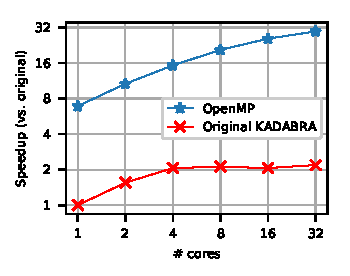
\includegraphics{sources/plots/betw-apx/original-vs-baseline.pdf}
\caption{Average speedup (preprocessing + ADS, geom.\ mean) of OpenMP baseline over
the original sequential implementation of \kadabra.}
\label{fig:betw-apx:original-vs-baseline}
\end{subfigure}\hfill
\begin{subfigure}[t]{.48\textwidth}
\centering
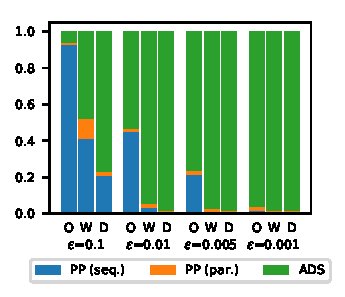
\includegraphics{sources/plots/betw-apx/time-breakdown.pdf}
\caption{Breakdown of sequential \kadabra running times into preprocessing and ADS
(in percent) on instances orkut-links~(O), wikipedia\_link\_de~(W), and
dimacs9-COL~(D)}
\label{fig:betw-apx:time-breakdown}
\end{subfigure}
\caption{Performance of OpenMP baseline.}
\end{figure}

In a first experiment, we compare our OpenMP baseline against the original
implementation of \kadabra (see \Cref{sec:betw-apx:first-attempts} for these two
approaches). We set the absolute approximation error to $\epsilon =
\numprint{0.01}$. The overall speedup (\ie both preprocessing and ADS) are
reported in \Cref{fig:betw-apx:original-vs-baseline}.
The results show that our OpenMP baseline outperforms the
original implementation considerably (by a factor of
$\onedigit{\adsSuDtVsOmp}\times$), even in a single-core setting.
%
This is mainly due to implementation tricks (see
\Cref{sec:betw-apx:kad-improvements}) and parameter tuning (as discussed in
\Cref{sec:betw-apx:balancing-costs}). Furthermore, for $32$ cores, our OpenMP
baseline performs $\onedigit{\overallSuOmpVsOriginal}\times$ better than the
original implementation of \kadabra\ -- or
$\onedigit{\adsSuOmpVsOriginal}\times$ if only the ADS phase is considered.
Hence, for the remaining experiments, we discard the original implementation as
a competitor and focus on the parallel speedup of our algorithms.

\subsection{Preprocessing and ADS Costs}
%
To understand the relation between the preprocessing and ADS phases of
\kadabra, we break down the running times of the OpenMP baseline
in \Cref{fig:betw-apx:time-breakdown}. In this plot, we present the fraction
of time that is spent on ADS on three exemplary instances and for different
values of $\epsilon$.
Especially if $\epsilon$ is small, the ADS running time dominates the overall
performance of the algorithm.
Thus, improving the scalability of the ADS phase is of critical importance.
For this reason, we neglect the preprocessing phase and only consider ADS when
comparing to our \localframe and \sharedframe algorithms.


\subsection{Parallel Speedup}
%
\begin{figure}[t]
\centering
\begin{subfigure}[t]{.48\textwidth}
\centering
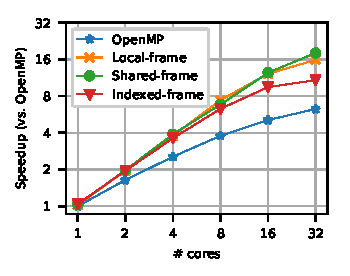
\includegraphics{sources/plots/betw-apx/parallel-speedup.pdf}
\caption{Average ADS speedup (geom.\ mean) of epoch-based
algorithms over sequential OpenMP baseline.}
\label{fig:betw-apx:parallel-speedup}
\end{subfigure}\hfill
\begin{subfigure}[t]{.48\textwidth}
\centering
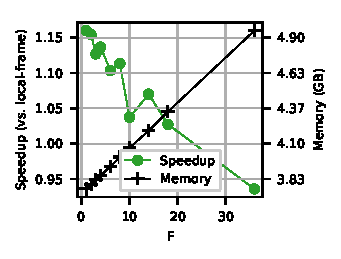
\includegraphics{sources/plots/betw-apx/time-memory.pdf}
\caption{Average ADS speedup (over 36-core \localframe, geom.\ mean)
and memory consumption of \sharedframe, depending on the number
of SFs.}
\label{fig:betw-apx:time-memory}
\end{subfigure}
\caption{Performance of epoch-based algorithms.}
\end{figure}

In \Cref{fig:betw-apx:parallel-speedup} we report the parallel
speedup of the ADS phase of our epoch-based algorithms
relative to the OpenMP baseline.
All algorithms are configured to check the stopping condition
after a fixed number of samples (see \Cref{sec:betw-apx:termination-latency}
for details). The number $F$ of SF pairs of \sharedframe
has been configured to $2$, which we found to be a good setting
for $T = 32$. On $32$ cores, \localframe and \sharedframe achieve
parallel speedups of $\onedigit{\adsParallelSuLf}\times$
and $\onedigit{\adsParallelSuSf}\times$; they both significantly
improve upon the OpenMP baseline, which can only
achieve a parallel speedup of $\onedigit{\adsParallelSuNaive}\times$
(\ie \localframe and \sharedframe are $\onedigit{\adsSuLfVsOmp}\times$
and $\onedigit{\adsSuSfVsOmp}\times$ faster, respectively;
they also outperform the original implementation by
factors of $\onedigit{\adsSuLfVsOriginal}\times$ and
$\onedigit{\adsSuSfVsOriginal}\times$, respectively).
%
The difference between \localframe and \sharedframe is insignificant
for lower numbers of cores; this is explained by the fact that the reduced
memory footprint of \sharedframe only improves performance once memory
bandwidth becomes a bottleneck. For the same reason, both algorithms
scale very well until $16$ cores; due to memory bandwidth limitations,
this nearly ideal scalability does not extend to $32$ cores.
This bandwidth issue is known to affect graph traversal algorithms
in general~\cite{DBLP:conf/icpp/BaderCF05,DBLP:journals/ppl/LumsdaineGHB07}.

\subsection{Indexed-frame Algorithm}
\label{sec:betw-apx:exp-indexed-frame}
%
The \indexedframe algorithm is not as fast as \localframe and \sharedframe on
the instances depicted in \Cref{fig:betw-apx:parallel-speedup}; it achieves a
parallel speedup of $\onedigit{\adsParallelSuDt}\times$ on $32$ cores. However,
it is still considerably faster than the OpenMP baseline (by a factor of
$\onedigit{\adsSuDtVsOmp}\times$). There are two reasons why the determinism of
\indexedframe is costly: \indexedframe has similar bandwidth requirements as
\localframe; however, it has to allocate more memory as SFs are buffered for
longer periods of time. On the other hand, even when enough samples are
collected, the stopping condition has to be checked on older samples first,
while \localframe and \sharedframe can just check the stopping condition on the
most recent sampling state.

\subsection{Impact of Parameter $F$}
%
In a final experiment, we evaluate the impact of the parameter $F$ of
\sharedframe on its performance. Note that this experiment also
demonstrates the difference in memory consumption of \sharedframe
($F \in \set{1, \ldots, T}$) and \localframe (equivalent to
$F = T$). \Cref{fig:betw-apx:time-memory} depicts the results.
%
The experiment is done with $36$ cores; hence, memory pressure
is even higher than in the previous experiments.
The plot demonstrates that, in this situation, minimizing the
memory bandwidth requirements at the expense of synchronization
overhead is a good strategy. Hence, for larger number of cores,
we can minimize memory footprint and maximize performance
at the same time.

\section{Related Work}
\label{sec:betw-apx:related-work}
%
\paragraph{ADS Algorithms}
%
Our parallelization strategy can be applied to arbitrary ADS algorithms. ADS
was first introduced by Lipton and Naughton to estimate the size of the
transitive closure of a digraph~\cite{DBLP:conf/vldb/LiptonN89}. It is used in
a variety of fields, \eg in statistical
learning~\cite{DBLP:conf/kdd/ProvostJO99}.
%
In the context of betweenness centrality, ADS has been used to approximate
distances between pairs of vertices of a graph~\cite{oktay2011distance}, to
approximate the $\betw(\cdot)$ value of the vertices in a
graph~\cite{DBLP:conf/waw/BaderKMM07,DBLP:conf/waw/BaderKMM07,DBLP:journals/tkdd/RiondatoU18},
and to approximate the betweenness centrality of a single
vertex~\cite{DBLP:journals/corr/abs-1810-10094}. An analogous strategy is
exploited by Mumtaz and Wang~\cite{DBLP:conf/cikm/MumtazW17} to find
approximate solutions to the group-betweenness maximization problem.

\paragraph{Betweenness Centrality Approximation Algorithms}
%
Regarding more general (\ie not necessarily ADS) algorithms
for $\betw(\cdot)$, a survey from Matta \etal~\cite{matta2019comparing}
provides a detailed overview of the state of the art.
The \rk~\cite{DBLP:journals/datamine/RiondatoK16} algorithm represents the
leading non-adaptive sampling algorithm for betweenness centrality approximation;
\kadabra was shown to be $100\times$ faster than \rk in undirected real-world
graphs, and $70\times$ faster thank \rk in directed graphs~\cite{DBLP:conf/esa/BorassiN16}
McLaughlin and Bader~\cite{DBLP:conf/sc/McLaughlinB14} introduced a work-efficient parallel
algorithm for betweenness centrality approximation, implemented for single- and multi-GPU
machines. Madduri \etal~\cite{DBLP:conf/ipps/MadduriEJBC09} presented a lock-free
parallel algorithms optimized for specific massively parallel non-x$86\_64$ architectures
to approximate or compute $\betw(\cdot)$ exactly in massive networks.
Unlike our approach, this lock-free algorithm parallelizes the collection of individual
samples and is thus only applicable to betweenness centrality and not to general
ADS algorithms. Additionally, according to the authors of~\cite{DBLP:conf/ipps/MadduriEJBC09}
this approach hits performance bottlenecks on x$86\_64$ even for $4$ cores.

\paragraph{Concurrent Data Structures}
%
The SFs used by our algorithms are concurrent data structures that enable us to minimize
the synchronization latencies in multi-threaded environments.
Devising concurrent (lock-free) data structures that scale over multiple cores is not
trivial and much effort has been devoted to this
goal~\cite{DBLP:conf/osdi/Boyd-WickizerCMPKMZ10,DBLP:journals/tpds/Michael04}.
A well-known solution is the Read-Copy-Update mechanism (RCU); it was introduced
to achieve high multi-core scalability on read-mostly data
structures~\cite{mckenney1998read}, and was leveraged by several
applications~\cite{DBLP:conf/podc/ArbelA14,DBLP:conf/asplos/ClementsKZ12}.
Concurrent hash tables are another popular example~\cite{DBLP:conf/sosp/DavidGT13}.

\section{Conclusions}
%
In this chapter, we observed that previous techniques to
parallelize ADS algorithms are insufficient to scale to large numbers of
threads. However, we found that significant speedups can be achieved by
employing adequate concurrent data structures. Using such data structures in
connection with our new epoch-based mechanism, we were able to devise parallel
ADS algorithms that, in our betweenness centrality case study, consistently
outperform the state of the art but also achieve different trade-offs between
synchronization costs, memory footprint, and determinism of the result.

Sampling-based strategies are used to estimate other centralities such as
closeness~\cite{DBLP:journals/ijbc/BrandesP07,DBLP:journals/jgaa/EppsteinW04},
group betweenness~\cite{DBLP:conf/ipps/MadduriEJBC09}, electrical
closeness~\cite{DBLP:conf/esa/AngrimanPGM20}, or (group-) forest
closeness~\cite{DBLP:conf/sdm/GrintenAPM21}. Hence, regarding future work, a
promising direction for our algorithms is to adapt them to approximate other
centrality measures beyond betweenness.
